%%%%%%%%%%%%%%%%%%%%%%%%%%%%%%%%%%%%%%%%%%%%%%%%%%%%%%%%%%%%%%%%%%%
%TO AVOID FORMATTING ISSUES, COMPILE THIS ONLY AT WWW.OVERLEAF.COM%
%%%%%%%%%%%%%%%%%%%%%%%%%%%%%%%%%%%%%%%%%%%%%%%%%%%%%%%%%%%%%%%%%%%
%AUTHOR: ABHINAV BAKSHI
%CLASS:  BE C 302
%%%%%%%%%%%%%%%%%%%%%%%%%%%%%%%%%%%%%%%%%%%%%%%%%%%%%%%%%%%%%%%%%%%
\documentclass[a4paper,12pt]{article}
\usepackage{graphicx}
%To use this font, you need XeTex or LuaTex, prefer openleaf
\newenvironment{codefont}{\fontfamily{ccr}\selectfont}{\par}

\title{
	\normalfont \normalsize 
	\textsc{Pimpri Chinchwad College of Engineering \\ 
		Computer Laboratory - IV} \\
	[10pt] 
	\rule{\linewidth}{0.5pt} \\[6pt] 
	\huge Assignment No - B4 \\
	\rule{\linewidth}{2pt}  \\[10pt]
}
\author{}
\date{\normalsize}


\begin{document}
\maketitle

%%%%%%%%%%%%%%%%%%%%%%%
% FOR A NUMBERED LIST
% \begin{enumerate}
% \item Your_Item
% \end{enumerate}
%%%%%%%%%%%%%%%%%%%%%%%
% FOR A BULLETED LIST
% \begin{itemize}
% \item Your_Item
% \end{itemize}
%%%%%%%%%%%%%%%%%%%%%%%
% TO IMPORT AN IMAGE
% \includegraphics[width=\textwidth]{name_of_file}
% \textwidth makes the picture the width of the paragraphs
%%%%%%%%%%%%%%%%%%%%%%%%%%%%%%
% TO CREATE A FIGURE WITH A NUMBER AND CAPTION
% \begin{figure}
% \includegraphics[width=\textwidth]{image}
% \caption{Your Caption Goes Here}
% \label{your_label}
% \end{figure}
% REFER TO YOUR FIGURE LATER WITH
% \ref{your_label}
% LABELS NEED TO BE ONE WORD
%%%%%%%%%%%%%%%%%%%%%%%%%%%%%
% TO ADD CODE
% \begin{codefont}
% Some code in "courier" font
%\end{codefont}
%%%%%%%%%%%%%%%%%%%%%%%%%%%%%
\section{Aim}
	\paragraph{} Write a program to check task distribution using Gprof.l.
	
\section{Objective}
	\begin{itemize}
		\item To check task distribution using Gprof.l
	\end{itemize}
	
\section{Software Requirements}
	\begin{itemize}
		\item	Linux
		\item	GCC
		\item   Gprof.l
	\end{itemize}
	
\section{Mathematical Model} 
	 Let 	 	 																	\\
	 S 	= 	{s, e, x, y, fme, DD, NDD, memshared} 									\\
	 S 	= 	Initial State 															\\
	 E 	= 	End State 																\\
	 X	= 	Input Value i.e. Executable files 										\\
	 Y	= 	Output i.e. Calculated time in milliseconds. 							\\
	 Fm 	= 	Main function i.e. test() function for the calculation of time. 	\\
	 DD 	= 	Deterministic data 													\\
	 NDD 	= 	Non-deterministic data 												\\
	 Memshared 	= 	Core that is used for execution i.e. core1/core2 				\\
	 
	
\section{Theory}
	\subsection{Gprof}
		\paragraph{} 
		\begin{itemize}
		\item Gprof is a performance analysis tool for Unix applications. It uses a hybrid of instrumentation and  sampling and was created as extended version of the older "prof" tool. Unlike prof, gprof is capable of limited call graph collecting and printing.\\
		\item GPROF was originally written by a group led by Susan L. Graham at the University of California, Berkeley for Berkeley Unix  Another implementation was written as part of the GNU project for GNU Binutils in 1988 by Jay Fenlason.
		\end{itemize}
	\subsection{Profiling Data File Format }
		\begin{itemize}
			\item The old BSD-derived file format used for profile data does not contain a magic cookie that allows to check whether a data file really is a gprof file. Furthermore, it does not provide a version number, thus rendering changes 	to the file format almost impossible. gnu gprof uses a new file format that provides these features. For backward compatibility, gnu gprof continues 	to support the old BSD-derived format, but not all features are supported with it. For example, basic-block execution counts cannot be accommodated by the old file format.\\ 
	\subsection{Insert gprof Command Summary :}\\
			After you have a profile data file gmon.out, you can run gprof to 			interpret the information in it. The gprof program prints a flat profile and 			a call graph on standard output. Typically you would redirect the output of 			gprof into a file with $>$. 
			
    \subsection{You run gprof like this:}\\
			gprof options [executable-file [profile-data files...]] [$> $outfile].
			If you omit the executable file name, the file a.out is used. If you give no    			profile data file name, the file gmon.out is used. If any file is not in the 			proper format, or if the profile data file does not appear to belong to the 			executable file, an error message is printed. 
			
	\subsection{Debugging gprof:}\\
			If gprof was compiled with debugging enabled, the `-d' option triggers debugging output (to stdout) which can be helpful in understanding its operation. The debugging number specified is interpreted as a sum of the following options: 
			
			2 - Topological sort :
			Monitor depth-first numbering of symbols during call graph analysis 
			4 – Cycles :
			Shows symbols as they are identified as cycle heads 
			16 – Tallying :
			As the call graph arcs are read, show each arc and how the total calls to each function are     	  		tallied 
			
			32 - Call graph arc sorting :
			Details sorting individual parents/children within each call graph entry 
			64 - Reading histogram and call graph records :
			Shows address ranges of histograms as they are read, and each call graph arc 
			128 - Symbol table :
			Reading, classifying, and sorting the symbol table from the object file. For line-by-line profiling (`-l' option), also shows line numbers being assigned to memory addresses. 
			256 - Static call graph :
			Trace operation of `-c' option 
			
		
		\end{itemize} 
		
		\newpage
		
\section{Implementation:}
    
	\paragraph{}
	\begin{itemize}
		 Instrumentation code is automatically inserted into the program code during compilation (for example, by using the '-pg' option of the gcc compiler), to gather caller-function data. A call to the monitor function 'mcount' is inserted before each function call.\\
       	Sampling data is saved in 'gmon.out' or in 'progname.gmon' file just before the program exits, and can be analyzed with the 'gprof' command-line tool. Several gmon files can be combined with 'gprof -s' to accumulate data from several runs of a program.\\
	   GPROF output consists of two parts: the flat profile and the call graph. The flat profile gives the total execution time spent in each function and its percentage of the total running time. Function call counts are also reported. Output is sorted by percentage, with hot spots at the top of the list.\\
   	The second part of the output is the textual call graph, which shows for each function who called it (parent) and who it called (child subroutines). There is external tool called gprof2dot capable of converting the call graph from gprof into graphical form.\\\\
   	\\

\section{Testing}   	
\subsection{Positive Testing}
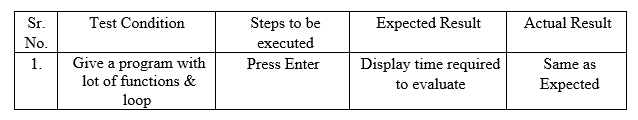
\includegraphics[width=\textwidth]{gprof_positive}

\subsection{Negative Testing}
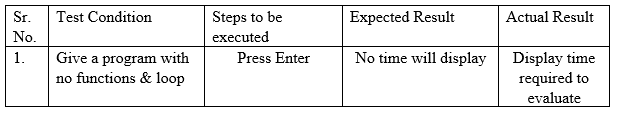
\includegraphics[width=\textwidth]{gprof_negative}
\newpage   	
   	
\section{Limitations and Accuracy:}
   	\paragraph{} 
   	\begin{itemize}
   		At run-time, timing values are obtained by statistical sampling. Sampling is done by probing the target program's program counter at regular intervals using operating system interrupts (programmed via profil(2) or setitimer(2) syscalls).\\
   		The resulting data is not exact, rather a statistical approximation. The amount of error is usually more than one sampling period. If a value is n times the sampling period, the expected error in the value is the square root of n sampling periods.\\
   		A typical sampling period is 0.01 second (10 milliseconds) or 0.001 second (1 ms) or in other words 100 or 1000 samples per second of CPU running time.\\
   	\end{itemize}
\section{Conclusion}
	\paragraph{} Hence we have successfully run the program using GPROF profiling tool.
\vspace{20px}
\begin{center}
	\begin{tabular}
		{|c|c|c|c|}\hline
		{\bf Roll No.}		&{\bf Name of Student}		&{\bf Date of Performance}  				&{\bf Date of Submission}  \\ \hline
		{302}	&	{Abhinav Bakshi}& {3/2/16}	&  {10/2/16}\\ \hline
	\end{tabular}\\ 
\end{center}


\section{Output}
	pccoecomp@PC33:~$ cd Desktop/\\
	pccoecomp@PC33:~/Desktop$ cd gprof/\\
	pccoecomp@PC33:~/Desktop/gprof$ gcc -Wall -pg gprof.c\\ new_gprof.c -o gprofobj\\
	pccoecomp@PC33:~/Desktop/gprof$ ls\\
	analysis.txt  gmon.out  gprof.c   gprofobj   new_gprof~\\   Untitled Document~\\
	a.out         gprof     gprof.c~  gprof_obj  new_gprof.c\\
	pccoecomp@PC33:~/Desktop/gprof$ ./gprofobj \\
	\\
	Inside main()\\
	\\
	Inside func1 \\
	\\
	Inside new_func1()\\
	\\
	Inside func2\\ 
	\\
	Inside func3\\ 
	pccoecomp@PC33:~/Desktop/gprof$ ls\\
	analysis.txt  gmon.out  gprof.c   gprofobj   new_gprof~\\   Untitled Document~\\
	a.out         gprof     gprof.c~  gprof_obj  new_gprof.c\\
	pccoecomp@PC33:~/Desktop/gprof$ gprof gprofobj gmon.out >\\ analysis.txt\\
	pccoecomp@PC33:~/Desktop/gprof$ ls\\
	analysis.txt  gmon.out  gprof.c   gprofobj   new_gprof~\\   Untitled Document~\\
	a.out         gprof     gprof.c~  gprof_obj  new_gprof.c\\
	pccoecomp@PC33:~/Desktop/gprof$ \\
	\\

\section{Plagarism Report}
	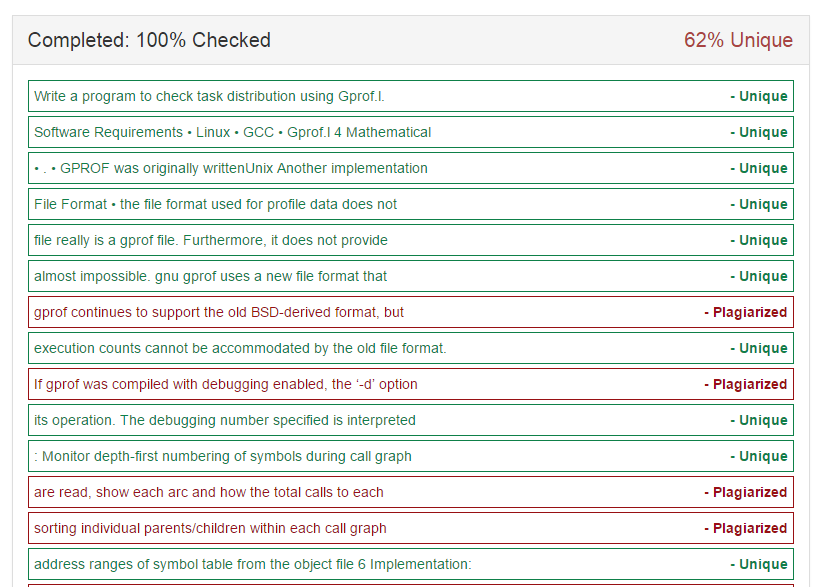
\includegraphics[width=\textwidth]{gprof_plaga}
\end{document}
 

 
